%%%%%%%%%%%%%%%%%%%%%%%%%%%%%%%%%%%%%%%%%%%%%%%%%%%%%%%%%%%%%%%%%%%%%%%%
%    INSTITUTE OF PHYSICS PUBLISHING                                   %
%                                                                      %
%   `Preparing an article for publication in an Institute of Physics   %
%    Publishing journal using LaTeX'                                   %
%                                                                      %
%    LaTeX source code `ioplau2e.tex' used to generate `author         %
%    guidelines', the documentation explaining and demonstrating use   %
%    of the Institute of Physics Publishing LaTeX preprint files       %
%    `iopart.cls, iopart12.clo and iopart10.clo'.                      %
%                                                                      %
%    `ioplau2e.tex' itself uses LaTeX with `iopart.cls'                %
%                                                                      %
%%%%%%%%%%%%%%%%%%%%%%%%%%%%%%%%%%
%
%
% First we have a character check
%
% ! exclamation mark    " double quote  
% # hash                ` opening quote (grave)
% & ampersand           ' closing quote (acute)
% $ dollar              % percent       
% ( open parenthesis    ) close paren.  
% - hyphen              = equals sign
% | vertical bar        ~ tilde         
% @ at sign             _ underscore
% { open curly brace    } close curly   
% [ open square         ] close square bracket
% + plus sign           ; semi-colon    
% * asterisk            : colon
% < open angle bracket  > close angle   
% , comma               . full stop
% ? question mark       / forward slash 
% \ backslash           ^ circumflex
%
% ABCDEFGHIJKLMNOPQRSTUVWXYZ 
% abcdefghijklmnopqrstuvwxyz 
% 1234567890
%
%%%%%%%%%%%%%%%%%%%%%%%%%%%%%%%%%%%%%%%%%%%%%%%%%%%%%%%%%%%%%%%%%%%
%
\documentclass[12pt]{iopart}
\usepackage{graphicx,epstopdf}
\usepackage{caption}
\usepackage{subcaption}
\usepackage{lscape}
\usepackage{hyperref}
\graphicspath{ {./figs/} }
%Uncomment next line if AMS fonts required
%\usepackage{iopams}
\begin{document}

\title[Neural Co-Processors]
{Neural Co-Processors for Restoring Brain Function:\\Results from a Cortical Model of Grasping}

% Authorship temporarily removed for double-anonymous review
\author{Matthew J Bryan$^{1}$, Linxing Preston Jiang$^{1}$, Rajesh P N Rao$^{1}$}

\address{$^{1}$ Neural Systems Laboratory, Paul G. Allen School of Computer
Science \& Engineering, University of Washington, Box 352350,
Seattle, WA 98105, USA}

\ead{\{mmattb,prestonj,rao\}@cs.washington.edu}
\vspace{10pt}
\begin{indented}
\item[]November 2022
\end{indented}

\begin{abstract}
\textit{Objective} A major challenge in closed-loop brain-computer interfaces (BCIs)
is finding optimal stimulation patterns as a function of ongoing neural activity for
different subjects and for different objectives. Traditional approaches, such as
those currently used for deep brain stimulation (DBS), have largely followed a manual
trial-and-error strategy to search for effective open-loop stimulation parameters,
a strategy that is inefficient and does not generalize to closed-loop
activity-dependent stimulation.
\textit{Approach} To achieve goal-directed closed-loop neurostimulation, we propose
the use of brain co-processors, devices which exploit artificial intelligence (AI)
to shape neural activity and bridge injured neural circuits for targeted repair and
rehabilitation.  Here we investigate a specific type of co-processor called a ``neural
co-processor'' which uses artificial neural networks (ANNs) and deep learning to learn optimal
closed-loop stimulation policies. The co-processor adapts the stimulation policy as
the biological circuit itself adapts to the stimulation, achieving a form of brain-device
co-adaptation. We tested the neural co-processor's ability to restore function after
stroke by simulating a variety of lesions in a previously published cortical model
of grasping.  We additionally tested the ability of our co-processor
to adapt its stimulation as the simulated cortical network and simulated sensors
underwent changes.
\textit{Main results} Our results show that a neural co-processor can restore
reaching and grasping function after a simulated stroke in a cortical model, achieving
recovery towards healthy function in the range 75-90\%. Our co-processor successfully
co-adapted to accomplish the reach-and-grasp task after a variety of lesions to the
simulated cortical circuit.
\textit{Significance} Our results provide the first proof-of-concept demonstration,
using computer simulations, of a neural co-processor for activity-dependent closed-loop
neurosimulation for optimizing a rehabilitation goal after injury. Our results provide
insights on how such co-processors may eventually be developed for \textit{in vivo} use
to learn complex adaptive stimulation policies for a variety of neural rehabilitation
and neuroprosthetic applications. 
\end{abstract}

\vspace{2pc}
\noindent{\it Keywords}: brain-computer interface, neural co-processor, AI, machine learning, deep learning, neural networks, stimulation, computational models
%
% Uncomment for Submitted to journal title message
%\submitto{\JPA}
%
% Uncomment if a separate title page is required
\maketitle
% 
% For two-column output uncomment the next line and choose [10pt] rather than [12pt] in the \documentclass declaration
%\ioptwocol
%



\section{Introduction}
Brain-computer interfaces (BCIs) have made significant advances over the last several decades, leading
to the control of a wide variety of virtual and physical prostheses through neural signal decoding
\cite{rao.bcibook, wolpaw.bcibook, moritz.neuro, lebedev.bmi}. Separately, advances in stimulation techniques and modeling have allowed
us to probe neural circuit dynamics (e.g. \cite{walker.inception}) and learn to better drive neural
circuits towards desired target dynamics by encoding and delivering information through
stimulation \cite{niparko.cochlear, weiland.retinal, tomlinson.propr, tabot.tact, tyler.tact,
dadarlat.tact, sharlene.tact, cronin.tact}. Bi-directional BCIs (BBCIs) allow stimulation to be
conditioned on decoded brain activity and encoded sensor data for applications such as real-time,
fine-grained control of neural circuits and prosthetic devices (e.g., \cite{nicolelis.bmbi}).

Motivated by these advances, we investigate here a flexible framework for combining encoding
and decoding using ``neural co-processors'' \cite{rao.coproc}, a type of brain co-processor \cite{rao.braincoproc}. Neural co-processors leverage artificial neural networks (ANNs) and deep
learning to compute optimal closed-loop stimulation patterns. The approach can be used to not only drive neural activity
toward desired activity regimes, but also to achieve task goals external to the subject, such as finding closed-loop
stimulation patterns for motor cortical neurons for restoring the ability to reach and grasp an object. Likewise, the
framework generalizes to stimulation based on both brain activity and external sensor measurements, e.g., from cameras or
light detection and ranging (LIDAR) sensors, in order to restore perception (e.g., cortical visual prosthesis) or
incorporate feedback for real-time prosthetic control (see \cite{rao.braincoproc} for details).

The co-processor framework also allows co-adaptation with biological circuits in the brain by updating its stimulation policy, while the brain updates its own response to the stimulation via adaptation and neural plasticity, or updates due to other reasons. This allows the co-processor to continually optimize its outputs for the desired optimization function in the presence of significant non-stationarity in the brain.

Here we use computer simulations to demonstrate a neural co-processor that restores
movement in a computational model of cortical networks controlling a limb, after a simulated stroke affects the ability to
use that limb. Our demonstration combines:
\begin{itemize}
	\item An emulation model based on ANNs, which models the relationship between 
	      stimulation, decoded brain activity, and task performance.
	\item An AI agent based on ANNs which determines the best stimulation to apply in a closed-loop fashion in real time.
\end{itemize}

\section{Background}
Significant advances have been made in understanding and modeling the effects of electrical stimulation
on the brain. Researchers have explored how information can be biomimetically or
artificially encoded and delivered via stimulation to neuronal networks in the brain and
other regions of the nervous system for auditory \cite{niparko.cochlear}, visual \cite{weiland.retinal},
proprioceptive \cite{tomlinson.propr}, and tactile
\cite{tabot.tact, tyler.tact, dadarlat.tact, sharlene.tact, cronin.tact} perception.
Advances have also been made in modeling the effects of stimulation over large scale, multi-region
networks, and across time \cite{shanechi.stimmodel}. Some models can additionally adapt to ongoing
changes in the brain, including changes due to the stimulation itself
\cite{tafazoli.acls}. For our simulations described below, we use a stimulation
model, not unlike those cited above, which seeks to account for both network dynamics
and non-stationarity. In addition to training the model to have a strong ability to predict
the effect of stimulation, we additionally adapt it to be useful for learning an
optimal stimulation policy, a property distinct from predictive
power alone.

Researchers have also explored both open- and closed-loop stimulation protocols for
treating a variety of disorders. Open loop stimulation has been effective in
treating Parkinson's Disease (PD) \cite{benabid.parkinsons}, as well as various
psychiatric disorders \cite{holtzheimer.psy, kisely.psy, fraint.psy}.
In research more directly related to our work, Khanna et al. \cite{khanna.openloop}, investigated 
the use of open loop stimulation in restoring dexterity after a lesion in a nonhuman primate's (NHP's) motor cortex.
The authors demonstrate that the use of low-frequency alternating current, applied epidurally,
can improve grasp performance.

While open loop stimulation techniques have yielded clinically useful results, results in other domains have been mixed, such as in visual
prostheses \cite{bosking.visual}, and in invoking somatosensory feedback
\cite{cronin.tact}. We believe this is due to the stimulation not being conditioned
on the ongoing dynamics of the neural circuit being stimulated. From moment to moment and
throughout the day, a neuronal circuit in the brain can be expected to respond differently even when the same stimulation parameters are used,
due to the multitude of different external and internal inputs influencing the circuit's ongoing activity. Stimulation
therefore needs to be proactively adapted in response. This need is even
greater over longer time scales as the effects of plasticity, changes in clinical conditions, and ageing change
the dynamics and connectivity of the brain. Closed-loop stimulation may also provide means
to better regulate the energy use of an implanted stimulator, allowing it to
intelligently regulate when to apply stimulation, in order to preserve implant
battery life. Another benefit is that closed-loop stimulation offers an opportunity to minimize the 
side-effects of stimulation, through real time regulation
of the stimulation parameters, such as in the use of deep brain stimulation (DBS) in
PD patients \cite{little.park}. In recent years, closed-loop stimulation has been used to aid in learning
new memories after some impairment \cite{berger.closedloop, kahana.biomarker},
to replay visually-invoked activations \cite{tafazoli.acls}, and for optogenetic
control of a thalamocortical circuit \cite{bolus.opto}, among others.

A major open question is: how does one leverage closed-loop control for real-time
co-adaptation with the brain to accomplish an external task? ``Co-adaptation'' here refers
to the ability of a BCI to adapt its stimulation regime to the ongoing
changes in the circuit it is stimulating, and to adapt with that circuit to accomplish
the external task (e.g., grasping). The neural co-processor we present here provides one
potential model for accomplishing that. Through the use of deep learning, a neural 
co-processor model co-adapts its AI, which governs the
stimulation, with the neural circuit being stimulated.

For a neurologically complex task such as grasping, it is not possible to design
\textit{a priori} a fixed real-time controller for the (potentially impaired) neural circuits involved in the task. That is
due in large part to the variability of circuits from subject-to-subject,
as well as variations in the placement of sensors and stimulators in the
brain. The only plausible path to implementing a real-time controller is therefore to allow the device to adapt to the subject,
long-term changes in their brain activities, and variability in the sensors, stimulators and hardware. Our proposed neural
co-processors seek to accomplish such adaptation through ANNs and deep learning.

To gain insights into neural co-processors before testing them in \textit{in vivo} experiments, we investigated a number of crucial design elements through the use of a neural network model of the cortical areas involved in 
grasping, presented previously by Michaels et al. \cite{michaels.mrnn}. We
explored what properties of the co-processor allow
successful adaptation to the short-term dynamics of the cortical model as it is being stimulated,
as well as adaptation to longer-term connectivity changes in the cortical model.
We present a training method for neural co-processors for learning optimal stimulation patterns that drive improvements in external task performance,
while also adapting to the non-stationarity of the brain.

\section{Methods}

\begin{figure}
    \centering
    \begin{subfigure}[c]{0.75\textwidth}
		\centering
		\includegraphics[width=\textwidth]{weill_arch.png}
		\caption{}
	\end{subfigure}
	\hfill
    \begin{subfigure}[c]{0.75\textwidth}
		\centering
		\includegraphics[width=\textwidth]{cpn_michaels_arch_labeled.png}
		\caption{}
	\end{subfigure}
	\hfill
    \caption{{\bf Neural co-processor for restoring function after a brain injury}.
    An artificial neural network called the “Co-Processor Network” (CPN) is used to
    map input neural activity patterns in an area A to output stimulation patterns
    in same or other areas B in order to achieve a neural or behavioral goal using
    another ANN, an “Emulator Network” (EN) - see text for details. (a) The example
    here shows the CPN creating a new information processing pathway between prefrontal
    cortex and motor cortex, bypassing an intermediate area affected by brain injury
    (e.g., stroke). Adapted from \cite{rao.coproc}, (b) Our current study involves a
    simulated cortical grasping circuit. The CPN and EN both receive simulated brain
    recordings, which are created according to a recording model (see Methods).
    The CPN outputs stimulation parameters, which are applied to the simulated
    grasping circuit, according to a stimulation model. The EN models the relationship between the
    stimulation, brain recordings, and external task.}
    \label{fig:arch}
\end{figure}

\subsection{Architecture Overview}
First, we present the architecture of our neural co-processor design. This design aims to solve two
fundamental challenges in using neural stimulation to improve external task performance.
First, to restore function for complex tasks, such as grasping, the mapping between
neural activity, such as the activity encoding the intention to grasp, and the stimulation patterns
to be applied to a downstream motor area to enable grasping cannot be pre-determined.
As a result, the co-processor must learn what stimulation pattern is appropriate for achieving the
external task. Unfortunately, in most cases, we do not know the optimal stimulation patterns to train
the co-processor. This is because stimulation shapes the nonlinear dynamics of circuits in the brain
in complex ways, leading to complex effects in external behavior. It is therefore not obvious what
stimulation patterns will produce a desired behavior. 

A neural co-processor attempts to solve these problems with a pair of artificial neural networks (ANNs)
(Fig.~\ref{fig:arch}):
\begin{itemize}
    \item a ``Co-Processor Network'' (CPN), which maps neural activity, and possibly
	      data from external sensors, to appropriate stimulation parameters.
    \item an ``Emulator Network'' (EN) which models the effect of stimulation on neural dynamics and
          behavior for the external task.
\end{itemize}

The CPN can be trained using the backpropagation algorithm, the workhorse of deep learning for training ANNs.
However, backpropagation requires the error between the output of the CPN and a desired output, and as
discussed above, we do not have the desired output stimulation pattern. We do however know what the desired
output behavior in a task should be, e.g., a particular kind of grasp for a particular object or a particular
type of neural activity in a brain area corresponding to healthy activity. We can therefore compute the error
between this desired behavior and the actual behavior caused by the CPN due to stimulation. How do we
backpropagate this error, which is external to the CPN, to update the parameters of the CPN?

We use a trained EN to backpropagate the external task error to the CPN. We train the EN to predict
task-relevant parameters - a prediction of muscle velocities in our case - given the stimulation
parameters output by the CPN and any measured neural activity. If the EN is trained to a sufficiently
high level of precision, it can be used as a function approximator mapping stimulation to task output.
When training the CPN, we treat the EN's output as the actual task output (e.g., actual grasp
parameters).  We backpropagate through the EN (without changing its weights) the error between
the EN's output and the desired task output and use this backpropagated error to train the
CPN (see Fig. \ref{fig:arch}). 

In our experiments, the EN was a single layer fully connected long short-term memory (LSTM) recurrent
neural network (RNN), with hyperbolic tangent ($tanh$) activations, and a linear readout. It has 87 LSTM neurons,
which was chosen somewhat arbitrarily as a function of the input and output vector sizes. We found varying this neuron
count did not drastically change results. Although other architectures could also be used, we found that this
LSTM architecture allows the EN to continuously adapt to long-running dependencies in the simulated neural dynamics, 
ar better than a vanilla RNN. The CPN had an almost identical architecture, but with 61 LSTM neurons. As with the CPN,
this neuron count was chosen as a function of the input and output vector sizes, but varying it upward had little effect on results.
There is no requirement for the EN and CPN to have similar network architectures, but we found that these choices worked
well in our experiments.

Note that the EN is more general than traditional models of neurostimulation which attempt to predict the effects of
stimulation on \em{neural activity}. The EN in a neural co-processor predicts the effects of stimulation (taking into
account ongoing neural dynamics) on \em{task performance}. This provides the key functionality needed to train the
CPN. In the special case where the task involves driving neural circuits in the brain to desired neural activities,
the EN reduces to more traditional models of stimulation.

For comparison, consider an EN architecture based on a traditional RNN with a nonlinearity. This is a nonlinear version
of the common linear time-invariant state space model of stimulation (see, e.g.,  \cite{shanechi.stimmodel}). 
We found, however, that compared to LSTM-based EN, the linear model and the traditional nonlinear RNN are both not
sufficiently powerful to capture the long-term dependencies in stimulation effects needed for the CPN to learn well.
Our use of an LSTM-based EN builds on previous work modeling biological neural networks for predicting local field potentials
\cite{kim.lstm}, and modeling stimulation \cite{guclu.lstm}.

\subsection{Simulation Overview}
To test the feasibility of the neural co-processor approach, we used a previously published model of a
grasping circuit in a nonhuman primate (NHP) brain. Using such a model allows us to explore some of the critical
architectural choices and training algorithms, enabling us to rapidly and cheaply iterate on our
design, prior to any \textit{in vivo} experiments. 

In the present study, we use the grasping network model of Michaels et al. \cite{michaels.mrnn}
(Fig.~\ref{fig:michaels}a). The network, representing multiple interconnected cortical areas, was trained
to mimic the grasping circuits of NHP subjects engaged in a delayed reach-to-grasp task.
The model's design draws on a body of literature focused on architectures and training methods for RNNs which
seek to create artificial neural networks with activation dynamics similar to biological circuits,
including circuits for delayed grasping tasks \cite{susillo.mrnn}. The model consists of three
``modular'' vanilla RNNs (mRNNs), representing the cortical areas AIP, F5 and M1 respectively, and a linear
readout layer (Fig.~\ref{fig:michaels}a). Each ``module'' consists of 100 vanilla
RNN neurons, with a nonlinearity applied on the outputs. The modules are internally fully connected,
and are connected to each other sparsely (10\% connectivity in our case). The inputs to the network are visual features
representing the object to be grasped, as well as a hold signal. The visual features
intend to capture the features represented in the subject's visual cortex. They were extracted using
VGGNet \cite{simonyan.vgg} from 3D renderings of the same objects which the subjects grasped. The hold signal is
a boolean which encodes the point in the experiment when the subject began to reach. The outputs of the
network are muscle length velocities for the shoulder, arm, and hand of the subject. The actual
velocities were captured with a motion capture glove, and the Michaels et al. network model 
was trained to recapitulate those grasping motions.\footnote{Data and trained models from this work
were supplied to us by the lead author of \cite{michaels.mrnn}. We re-implemented their model in PyTorch,
and used their trained parameters for an arbitrarily chosen subject.} 

\begin{figure}
	\centering
	\begin{subfigure}[c]{0.69\textwidth}
		\centering
		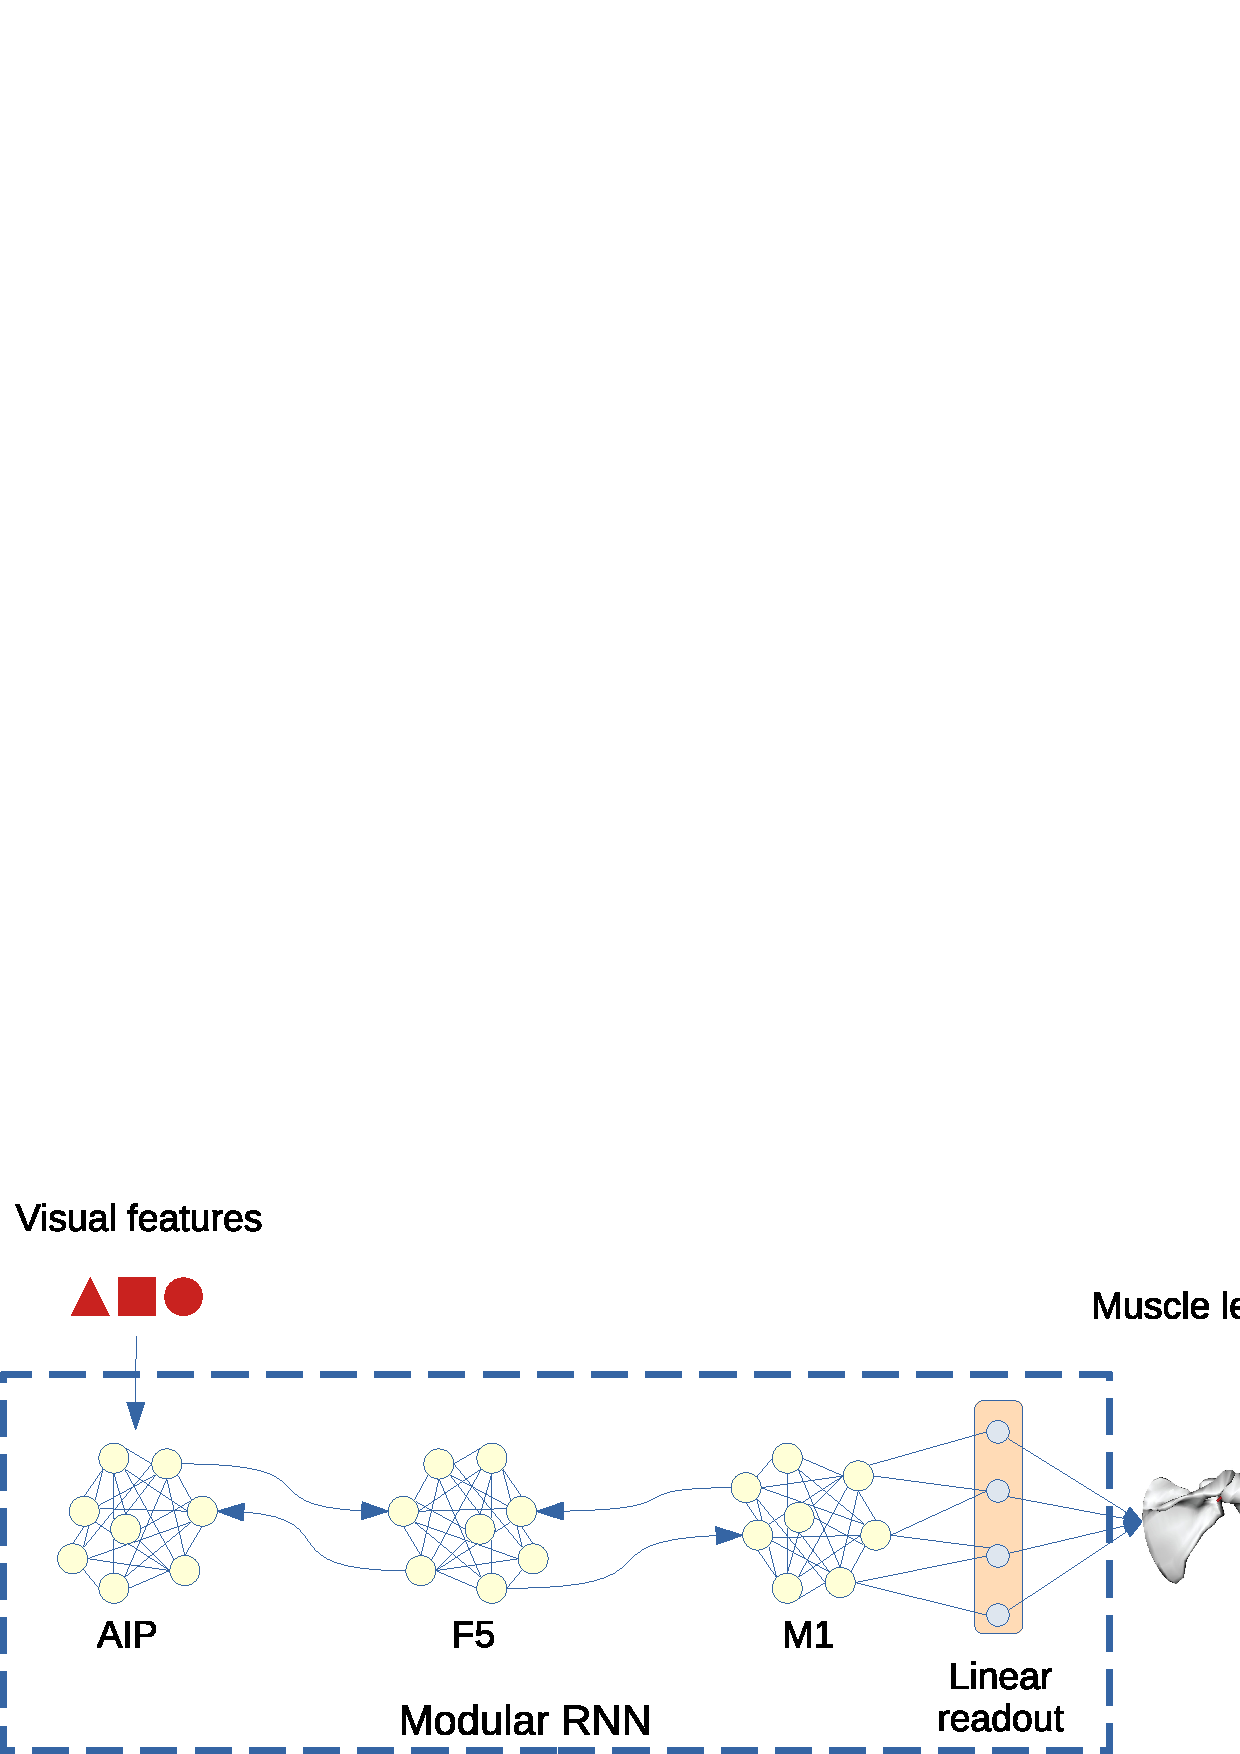
\includegraphics[width=\textwidth]{michaels.png}
		\caption{}
	\end{subfigure}
	\hfill
	\begin{subfigure}[c]{0.30\textwidth}
		\centering
		\includegraphics[width=\textwidth]{mRNN_J.png}
		\caption{}
	\end{subfigure}
	\hfill
\caption{\textbf{Architecture of the Brain Model.} (a) Modular RNN (mRNN) used by Michaels et al.
        \cite{michaels.mrnn} to model cortical circuits involved in grasping objects.
        The emergent dynamics of the three modules correspond well to neural activity in
        primate cortical areas AIP, F5, M1, respectively, for the same task. Visual
        features of an object (derived from VGGNet) propagate forward through the
		network, conditioning the grasp on the object's size and shape. (b)
		Connectivity matrix $J$. Connected neuron pairs are indicated in black, though the
		actual network weights are floating point values. White indicates non-connections.
		Note the within-module connections (black squares along	the diagonal) are fully
		connected while connections to adjacent modules are sparse
		($10\%$ of possible connections).}
\label{fig:michaels}
\end{figure}

The grasping model we use \cite{michaels.mrnn} implements a vision-to-grasp pipeline, from the visual
processing needed to move the hand to the appropriate position for the grasp to shaping the hand for
grasping an object of a particular shape. The emergent dynamics of the model's ``modules'', once trained,
correspond roughly to the responses in the cortical areas AIP, F5, and M1 in a NHP subject's brain.
Specifically, the activity of the first module (Fig.~\ref{fig:michaels}a), receiving the visual inputs in a trial resembles
the activity in area AIP of the NHP subject from the same trial. Likewise, the second and
third modules resemble the activity from the subjects's F5 and M1 cortical areas, respectively.
The emergent network dynamics show a number of other correspondences to the subjects' 
brain activity as well (see \cite{michaels.mrnn} for details). For convenience, we will refer to the three
modules in the model using the cortical areas (AIP, F5, M1) they correspond to. For details on how this network
was trained, refer to Supplementary Materials \ref{sup:michaelstraining}. For additional details on the task structure, see
Supplementary Materials \ref{sup:michaelstask}.

An important attribute of the grasping network model is that  the simulated circuit's activity shows a relatively
clear separation for different object shapes, i.e. the visual input to the network is leveraged by the model to
successfully generate hand shape trajectories for grasping objects of particular shapes, and sizes. As we will note
below, if the visual information is prevented from propagating through the modules, the model can at best learn a
grasp stereotyped across all object sizes and shapes. 

\subsubsection{Lesioning the model causes real world failure modes.}
Simulating a brain lesion in the grasping model described above results in error
modes which resemble some natural lesions of the primate brain. For example, a ``lesion''
involving zeroing some of the outputs of the first (AIP) module 
leads to a reaching motion generally succeeding, but finger muscle velocities show a high
degree of error - effectively implying that the subject can reach to grasp, but cannot
tailor the grasp to the current object. This is likely due to object shape information not
being fully conveyed to the motor cortex (M1) module. Such a form of hand muscle spasticity
is also a common symptom in certain strokes where the subject is able to position their
hand, but is unable to properly form the appropriate grasp \cite{khanna.openloop,
puthenveettil.hand}. 

On the other hand, if we lesion of a portion of the motor cortex (M1) module in the model,
we see a more complete loss of movement, affecting even the ability to reach for the grasp.
Finally, if we ``disconnect'' communication between the F5 and M1 modules, we see a
failure similar to an AIP lesion: the reaching movement is generally achieved, but we see
a disproportionate impact on forming the appropriate hand grasp. See Fig. \ref{fig:lesion}
for examples.

\begin{figure}[h]
	\centering
	\begin{subfigure}[c]{0.62\textwidth}
	    \centering
	    \includegraphics[width=\textwidth]{lesion_trajs.pdf}
	    \caption{}
	\end{subfigure}
	\hfill
	\begin{subfigure}[c]{0.32\textwidth}
	    \centering
	    \includegraphics[width=\textwidth]{lesion_hand.pdf}
	    \caption{}
	\end{subfigure}
	\hfill
	\caption{\textbf{Simulating strokes by lesioning different parts of the model 
	         lead to differential impact on grasping behavior.}
             (a) Example muscle trajectories before (orange) and after (blue)
             simulated stroke due to AIP, F5-M1 and M1 lesions for a shoulder
             muscle (top row) and a hand muscle (bottom row). Lesions which prevent
             a forward propagation of visual information tend to have a larger effect
             on hand pose (example EIP muscle shown) than on the shoulder, which is more
             involved in the reach motion (example TMAJ muscle shown). Lesions of M1
             tend to cause a significant task loss on both.
             (b) Ratio of hand muscle mean squared error (MSE) losses vs.
             overall MSE losses, for different lesion types. The loss is measured
             relative to the model's movement trajectories prior to the lesion.
             Average of all trials, with +/- 1 stdev shown.}
	\label{fig:lesion}
\end{figure}

Given a particular type of lesion in the model, the co-processor's task is to
generate the appropriate stimulation pattern given mRNN activities. The
co-processor thus seeks to effectively bridge across the lesion and deliver
stimulation to enable grasping behavior tailored to the current object's shape.

In our experiments, we studied our co-processor's performance on three types of
simulated lesions:
\begin{itemize}
	\item \textbf{Loss of AIP Neurons:} We force the output of some proportion of ``AIP''
	      neurons to zero, effectively removing them from the network. This results in some amount of 
	      loss of object shape information.
	\item \textbf{Loss of F5-M1 Connections:} We prevent the propagation of
	      information between the ``F5'' and ``M1'' modules, effectively representing a
	      severing of the connections between the two modules. Note that the connections are sparse
	      and run in both directions, and we lesion the connections in both directions.
	\item \textbf{Loss of M1 Neurons:} We force the output of some proportion of ``M1''
	      neurons to zero. Here, the lesion may make it impossible for the co-processor
	      to find a perfect solution, since the loss of M1 neurons may make it impossible to
	      activate muscles in the same ways. However, in Results we will see that some recovery
	      is possible.
\end{itemize}

\subsubsection{Simulated network exhibits long running and stable dynamics.}
To compute stimulation patterns that optimize for a task, the co-processor must
learn to adapt to the dynamics of the network it is stimulating. Biological neural
networks as well as our simulated grasping network exhibit long range changes in dynamics
due to stimulation. A perturbation of the network (i.e. due to stimulation) will cause
changes in neuronal activations long after the stimulation has been applied, sometimes far
from the site of stimulation. Our model of the cortical grasping network exhibits the same
behavior.

To illustrate this, suppose we apply a small, one-time perturbation
to the hidden states of 10 randomly chosen neurons in the output (M1) module at some point
in time during a trial. By repeating this experiment many times, we can understand what the
distribution of long-running effects tends to look like on the output muscle velocities.

In Fig.~\ref{fig:dynamics} we see that even a single, one-time perturbation in
the network has effects dozens of time steps later. Our co-processor will need to learn to take
these dynamics into account. As we will show in the next subsection, the problem our co-processor
faces in our simulations is in fact even harder than this since we also incorporate
a model of stimulation effects on the neural circuit which includes both spatial and temporal
smoothing.

\begin{figure}[h]
	\centering
	\begin{subfigure}[c]{0.48\textwidth}
	    \centering
	    \includegraphics[width=\textwidth]{perturbe_single_tmaj.pdf}
	    \caption{}
	\end{subfigure}
	\hfill
	\begin{subfigure}[c]{0.48\textwidth}
	    \centering
	    \includegraphics[width=\textwidth]{perturbe_dist_tmaj.pdf}
	    \caption{}
	\end{subfigure}
	\hfill
	\begin{subfigure}[c]{0.48\textwidth}
	    \centering
	    \includegraphics[width=\textwidth]{perturbe_single_eip.pdf}
	    \caption{}
	\end{subfigure}
	\hfill
	\begin{subfigure}[c]{0.48\textwidth}
	    \centering
	    \includegraphics[width=\textwidth]{perturbe_dist_eip.pdf}
	    \caption{}
	\end{subfigure}
	\hfill
	\caption{\textbf{Perturbations of the simulated cortical network (i.e. due to stimulation)
	         have long-running effects on muscle activation.} Our results are consistent with
	         the fixed point analysis of the network in \cite{michaels.mrnn}, showing that the network
	         exhibits stability. It tends towards the original trajectory after perturbation.
	         Instantaneous random perturbation of a random group of 10 M1
	         neurons performed at time t=2s. (a, c) Single trial example for TMAJ, EIP muscles
	         respectively. (b, d) Distribution of effects across n=1000 samples on TMAJ, EIP muscles
	         respectively. Probability distribution shown to +/- 2 stdevs. Network exhibits similar
	         behavior when perturbance is performed at other times.}
	\label{fig:dynamics}
\end{figure}

\subsubsection{Stimulation model.}
In our experiments, we stimulate neurons only in the output area (here M1) since the co-processor's
purpose is to improve external task performance, which it is able to do with
appropriate stimulation of the M1 output region of the network model. In a more general setting, it is
conceivable that a co-processor could stimulate other areas of the brain as well to improve task
performance downstream, or to probe the brain to better reveal the user's intent (i.e. object
shape), but we leave these directions to future work.

To make our stimulation model more realistic, rather than allowing stimulation to directly change the
output of single neurons, we simulated how stimulation may affect a network of neurons using a
model that incorporates aspects of both spatial and temporal smoothing. Our intent was not to create a
biophysical model of stimulation (our model does not arrange neurons in a volume to allow for such detailed
simulation). Instead, the stimulation model approximates the effects of in-vivo biological stimulation (e.g.
extracellular electrical stimulation) by diffusing the effects of stimulation across neural tissue space and time.
Including this model implies that our EN must approximate this stimulation function, in addition to approximating
the cortical dynamics of the brain and the mapping of those dynamics onto the grasping task. In Supplementary Materials
\ref{sup:passthrough}, we compare results to the case with no stimulation or recording function.

Specifically, we use a stimulation function $S$ which receives as input the stimulation parameter vector $\theta$
from the CPN. $S$ performs temporal smoothing using a simple exponential decay model by adding its current input to
an exponentially decaying sum of inputs that decays towards $0.0$ at some rate (see Equation ~\ref{eq:temporalstim} below).
The effect of stimulation is thus not instantaneous, but rather decays with time. Likewise, to approximate how charge
dissipates into a surrounding volume, we applied Gaussian smoothing to map $\theta$ (16-D in our experiments) to changes
in the activations of a large number of the simulated M1 neurons (100 neurons in our experiments). If we assume each element
of the $\theta$ represents the stimulation parameter for a single electrode, our Gaussian smoothing operation emulates how
stimulation may affect the neurons in its vicinity more than it affects neurons further away. To accomplish that, we assume
our model neurons are aligned along a spatial dimension arbitrarily and fix $\sigma=1.75$. 

The resulting equations defining our stimulation model are:

\begin{equation}
\alpha_{t} = \tau\alpha_{t-1} + \theta_{t-1} \label{eq:temporalstim}
\end{equation}
\begin{equation}
s_{t} = C\alpha_{t}
\end{equation}

\begin{itemize}
	\item $\alpha$: the 16 dimensional internal state 
        of the stimulation function
	\item $\tau$: our decay rate for temporal smoothing, which we set arbitrarily to $0.7$
	\item $C$: a fixed $100 \times 16$ Gaussian smoothing matrix containing a single 1-D Gaussian
	           in each column, to implement spatial smoothing and spread of stimulation to the
	           stimulated neural population. 
	\item $s_{t}$: the spatiotemporally smoothed stimulation vector whose elements denote how
	               much stimulation is applied to each neuron at time step $t$ (see
	               Equation~\ref{eq:neural-activation} below).
\end{itemize}

The governing equations of an mRNN with stimulation then become:

\begin{equation}
x_{t+1} = Jx_{t} + Iv_{t} + s_{t} + b
\label{eq:neural-activation}
\end{equation}
\begin{equation}
a_{t} = tanh(x_{t})
\end{equation}
\begin{equation}
y_{t} = La_{t} + l
\end{equation}

\begin{itemize}
	\item $x$: the hidden state of each model neuron
	\item $J$: recurrent weight matrix
	\item $I$: input weight matrix
    \item $v_{t}$: input 
	\item $b$: activation bias
	\item $L$, $l$: parameters of the linear readout layer
	\item $y_{t}$: the output of the network
\end{itemize}

\begin{figure}[h]
	\begin{subfigure}[c]{0.45\textwidth}
		\centering
		\includegraphics[width=\textwidth]{stim_single.png}
		\caption{$\sigma=1.875$}
	\end{subfigure}
	\hfill
	\begin{subfigure}[c]{0.45\textwidth}
		\centering
		\includegraphics[width=\textwidth]{stim_single2.png}
		\caption{$\sigma=2.875$}
	\end{subfigure}

	\caption{\textbf{Simulating the effects of stimulation on a recurrent network across space and time.} The stimulation model performs spatial and temporal smoothing of a 16-dimensional
	         vector of stimulation parameters $\theta$ onto 100 neurons in a recurrent network.
	         The 16 elements of the vector represent in-effect 16 electrodes located
	         evenly along a spatial dimension, along which the 100 neurons are arranged
	         arbitrarily. We show here the effects of two randomized $\theta$ with two respective smoothing
	         parameters $\sigma$. After $t=0$,
		     $\theta$ is the zero vector. Color values indicate the magnitude of the value summed into
		     each neuron's hidden state at that time step. }
	\label{fig:stim_single}
\end{figure}

Fig. \ref{fig:stim_single} depicts an example where
$\theta$ is non-zero at $t=0$ and zero for all other times, illustrating the effects of 
stimulation on the network across space and time.  Fig. \ref{fig:stim_and_obs} illustrates the
effects of stimulation during a stroke simulation. In this case, the trial is one where $50\%$
of M1 neurons have been  lesioned (their outputs are zero), the inputs to the CPN are from the
AIP and F5 modules, and stimulation is applied to the M1 module. 

\begin{figure}[h]
	\centering
	\includegraphics[width=\textwidth]{stim_and_obs.png}
	\caption{\textbf{Example of stimulation and recording for a single trial.} Here, M1
	has been lesioned 50\%, indicated by hidden states of M1 neurons with a value of zero (bottom
	left panel, lowest part of the plot) . We record neural activities (recording model) only
	from the AIP and F5 modules, as explained in Section \ref{sec:experiments}. Stimulation is applied
	to M1 to drive the network's output. Stimulation is mostly constant until approximately t=275,
	when the hold signal was lifted and reach began.}
	\label{fig:stim_and_obs}
\end{figure}

\subsubsection{Recording model.}
To simulate recordings of our model neurons, we used a recording model that assumed the model neurons
are laid out along a single spatial dimension with the given number of electrodes spread evenly apart.
We then applied Gaussian convolution, where the Gaussian kernel is centered at each electrode position.
Thus, the recording from each `electrode' is a Gaussian-weighted average of the activities of all neurons
in the given module. Fig.~\ref{fig:stim_and_obs} (bottom panels) show an example of recordings obtained
using this recording model; note that the Gaussian-averaging of activities provides only a low-pass
filtered, potentially ambiguous view of the activities of the underlying neurons, making it more challenging
for the co-processor to interpret the neural activity and produce an appropriate stimulation pattern. Our
simulated recordings are similar in spirit, though not actually modeling, local field potentials recorded
extracellularly in biological neural tissue. In Supplemental section
\ref{sup:observability} we show that as we vary the observability of the
brain via this recording model the results are largely the same, up to a
point where objects can no longer be distinguished by the recording data.

\subsubsection{Simulating co-adaptation by the brain.}
To demonstrate the co-processor's ability to adapt with the brain as it adapts to the co-processor's
stimulation, we modify the cortical grasping network's parameters (synaptic weights and biases) throughout
the co-processor's training. We use the standard error backpropagation algorithm to adapt the grasping network
(using PyTorch's implementation of the $AdamW$ optimizer). With each trial, task loss is calculated and
backpropagated through the mRNNs as they receive stimulation. The learning rate was set arbitrarily
to a relatively low rate of $1\mathrm{e}{-7}$ so that the network adapts more slowly than the co-processor.

\subsubsection{Simulating recovery prior to co-processor use}
After a stroke, the human brain has the ability to learn and recover to some extent the behaviors
affected by the stroke. We simulated this ability in our grasping network model by re-training the
network for the grasping task after lesioning it. For our simulated lesions which zero
the outputs of neurons, the mRNN often cannot supply a partial recovery model.
This is because the mRNN model has sufficient redundancy built into it that lesioning it by
inactivating large numbers of neurons often leaves enough remaining degrees of freedom that a
nearly full recovery can occur, unless so many neurons are lesioned that no stimulation could be
effective.

In the case of a lesion that prevents communication between the F5 and M1 modules, information about
the input object's shape cannot propagate forward in the network to allow shaping of the hand for
grasping. However, the mRNN can learn a stereotyped grasp during the recovery period. After this recovery
period, a co-processor can further boost grasp accuracy by forward-propagating object shape information
from AIP and F5 to M1, acting as an artificial neural bridge. We explore this application of the
co-processor in one of our experiments below.

\subsubsection{Simulating a non-stationary recording function, e.g. sensor drift}
We also demonstrate the co-processor's ability to adapt to non-stationarity in the recording
function. Over time, implanted sensors may drift from true readings. To test the co-processor's
ability to adapt to that drift, we perform an experiment where the observation function
has a bias term which changes over time, according to a random process. Each epoch, we
add a random value to each element of the bias, drawn from a mean-0 Gaussian distribution. That
causes the ``sensors'' to have a drifting zero point over time.
See Supplementary Materials \ref{sup:drift} for further details.

\subsection{Training Paradigm}
\label{sec:training}

To train the CPN to generate appropriate stimulation patterns for grasping a given input object of a
particular shape, we can use the backpropagation algorithm to minimize the errors between the current
generated grasp and the desired target grasp. However, this error is in terms of grasp error instead of
error in stimulation patterns (which is what the CPN needs), and we have no way of backpropagating grasp
error through biological networks in the brain. This motivates our use of the EN as a model for the
transformation from stimulation to muscle velocities: we backpropagate grasp error through the EN,
while keeping its parameters fixed, and use this backpropagated error to change the parameters of the
CPN towards minimizing grasp error.

Using the EN to train the CPN requires careful interleaving of EN and CPN training epochs. EN training
epochs concentrate on updating the EN, based on observations of the effect of stimulation on the grasping
network model's output. The loss function when training the EN is the mean squared error (MSE) loss between
the EN's prediction and the  actual output of the grasping network (i.e. muscle velocities). During the CPN
training epochs, we keep the EN's parameters fixed and use the EN to train the CPN. Specifically, we
backpropagate the MSE loss between the EN's predicted output, and the desired output (target muscle velocities
for grasping the input object) through the CPN. Fig. \ref{fig:training} illustrates the EN and CPN training
processes.

\begin{figure}
	\centering
	\begin{subfigure}[c]{0.48\textwidth}
		\centering
		\includegraphics[width=\textwidth]{backprop_en.png}
		\caption{}
	\end{subfigure}
	\hfill
	\begin{subfigure}[c]{0.48\textwidth}
		\centering
		\includegraphics[width=\textwidth]{backprop_cpn.png}
		\caption{}
	\end{subfigure}
	\hfill
\caption{\textbf{Training the neural co-processor.} (a) EN training phase: 
         backpropagate actual vs predicted muscle velocity MSE loss.
         (b) CPN training phase: backpropagate actual vs target
         MSE loss, via EN, to CPN. This effectively treats the EN
         output as the actual, and thus the EN must be trained first.}
\label{fig:training}
\end{figure}

\subsubsection{Training and testing data sets.}
For training and evaluation of our model, we use the same data as in Michaels et al.
\cite{michaels.mrnn}, which was provided to us by the lead author. The data consist of:
\begin{itemize}
    \item The input visual features and hold signal. We input these to the simulated
          cortical circuit;
    \item The object identity. We use this to calculate how well the co-processor
          can differentiate objects; see Results section below;
    \item The muscle velocity data for the trial, as extracted from the data glove
          during the NHP trial, and as processed. This is our target output.
\end{itemize}

For each training session, we hold out a random sample of $20\%$ of the data to act as our validation data set; we
use the other $80\%$ for training.

\subsubsection{EN training.}
For the EN to be useful for training the CPN, it must accurately predict the behavioral effects of stimulation
produced by the CPN. In addition, backpropagating through the EN must yield gradients which are useful for
changing the weights of the CPN in order to produce better stimulation patterns or minimizing the error.
We discovered that this latter property does not occur simply by virtue of the former. Specifically, an EN
can be trained to high levels of predictive power, even for random stimulation, and to orders of magnitude
lower loss than the task loss, but backpropagation through the EN can still yield gradients which lead to
unstable training of the CPN. 

We hypothesize that the crux of the EN training problem is one of over-fitting: the EN may be trained
to achieve high predictive power on a data set of stimulation examples, but due to 
the high dimensionality of our stimulation parameters $\theta$, and the dynamics of the
network being stimulated, the function learned by the EN may be biased and provide gradients not suitable
for the stimulation inputs generated by the CPN during its training.

To address this problem, we first structure the training dataset for each EN training epoch
in a specific way. Each epoch, we include:
\begin{itemize}
	\item training examples using stimulation inputs generated by the current CPN;
	\item training examples using stimulation inputs generated by a small collection of CPNs obtained
	      by adding zero-mean Gaussian noise to the current CPN's parameters; and 
	\item training examples with white noise stimulation inputs.
\end{itemize}

Such a training paradigm is designed to cover a sufficient variety of examples to prevent overfitting,
and to do so in a way that explores the neighborhood of the current CPN's parameter space. Augmenting
a CPN-generated data set with white noise examples alone was not sufficient to stabilize CPN training,
but including additional examples generated by CPNs in the neighborhood of the current CPN helped train
the EN to perform well in that neighborhood and produce useful gradients for the CPN. ``Neighborhood''
here refers to the region of CPN parameter space near the current CPN. This may cause the EN to be
overfit, i.e. fit to the local area of CPN parameter space but exhibiting poor predictive power in
other areas of the space. However, we solve this problem by retraining the EN, interleaved with CPN
training. We show the effect of this dataset composition in one results section below
(\ref{sec:results_con}).

We composed each batch of EN training data as follows: \\

\begin{tabular}{|l|l|}
\hline
\textbf{Source}                                                                                                                            & \textbf{Proportion of dataset} \\ \hline
Data from current CPN                                                                                                       & 10\%                           \\ \hline
\begin{tabular}[c]{@{}l@{}}Data from current CPN with parameter noise\end{tabular} & 60\%                           \\ \hline
Data from white noise stimulation                                                                                                        & 30\%                           \\ \hline
\end{tabular} \\

Additionally, we use decoupled weight decay regularization \cite{loshchilov2017decoupled} to
mitigate overfitting, and a carefully chosen learning rate schedule. The schedule begins with
a higher learning rate initially ($4\mathrm{e}{-3}$), ramping down to a lower rate ($1\mathrm{e}{-4}$).
The learning schedule is based on the most recent prediction error on the validation portion of the
data set. We found that using rates much lower or higher than these rates in any training phase
may cause the EN learning to not converge. EN training proceeds until the network's output error
exceed a threshold, defined as a fraction of the current CPN's task loss. See Section
\ref{sec:interleaving} for further details on when we switch between training the EN and CPN.

\subsubsection{CPN training}
Once an EN is properly trained, we can use the EN as a surrogate for the part of the grasping model
that transforms stimulation patterns and neural activity to grasping behavior. We use a large number
of randomly sampled trials from the original Michaels et al. task \cite{michaels.mrnn} and generate
stimulation patterns using the current CPN alone. These stimulation patterns are passed through the EN
to generate predictions of output muscle velocities, which are compared to the desired target velocities
to compute the error. We backpropagate this error through the EN (without modifying its parameters) to
generate training gradients for the CPN. Fig.~\ref{fig:training} illustrates this training process.

We found that the CPN appears to train in two phases. In the first phase, it is largely learning the structure
of the reach-to-grasp task, e.g. that the muscles need to remain at a position during the hold period until the
reach begins. During this early training phase, the learning rate can be quite high ($1\mathrm{e}{-3}$). Later, the CPN
begins to learn the mapping between object shape information and the stimulation patterns needed to approximate
the target grasp for that object. This later phase of training requires a learning rate 2-3 orders of magnitude
lower than in the first phase ($1\mathrm{e}{-6} - 5\mathrm{e}{-5}$). See Section~\ref{sec:results} for more details.

\subsubsection{Interleaved CPN/EN training, and adapting to non-stationarity}
\label{sec:interleaving}
Having defined the training procedures for the EN and CPN, we can define a training
algorithm combining those two. We train the two in alternation, creating
a new EN each time we enter an EN training phase. We explored the possibility
of reusing an existing EN but found that retraining an EN was no more fast than training a new one.
Training a new EN also allows us to adapt to the brain's non-stationarity. That requires us to
determine when the current EN is no longer suitable for training the current CPN. 
Our algorithm retires the current EN and trains a new one when one of two conditions
is satisfied: (1) the EN's prediction error is sufficiently above some fraction of the CPN's task loss;
or (2) if CPN loss does not improve (or gets worse) over a sufficient number of recent training steps 
(this is a common stopping criterion in machine learning). Additional details can be found in the
Supplementary Materials section ~\ref{sup:encpninter}.

\subsection{Experiments}
\label{sec:experiments}

We performed 8 experiments to investigate the co-processor's ability to learn under a variety of
conditions: we studied three types of lesions to the grasping network (simulated stroke) and for
each lesion type, we either turned on or off brain co-adaptation, natural recovery before co-processor
use, and non-stationarity due to sensor drift. The following table summarizes the experiments
(a blank entry under a condition (e.g., Simulate co-adaptation?) means ``No'' while an X means ``Yes''): \\

\begin{table}[h]
\centering
\begin{tabular}{|l|l|c|c|c|}
\hline
 & \textbf{Lesion}                                           & \multicolumn{1}{l|}{\textbf{\begin{tabular}[c]{@{}l@{}}Simulate\\ co-adaptation?\end{tabular}}} & \multicolumn{1}{l|}{\textbf{\begin{tabular}[c]{@{}l@{}}Simulate\\ recovery?\end{tabular}}} & \multicolumn{1}{l|}{\textbf{\begin{tabular}[c]{@{}l@{}}Simulate\\ sensor\\ drift?\end{tabular}}}\\ \hline
1              & 50\% AIP loss                                             &                                                                                                 &                                                                                                &                                                                                                 \\ \hline
2              & 50\% AIP loss                                             & X                                                                                               &                                                                                                &                                                                                                 \\ \hline
3              & 50\% M1 loss                                              &                                                                                                 &                                                                                                &                                                                                                 \\ \hline
4              & 50\% M1 loss                                              & X                                                                                               &                                                                                                &                                                                                                 \\ \hline
5              & 100\% connection loss F5\textless{}-\textgreater{}M1 &                                                                                                 &                                                                                                &                                                                                                 \\ \hline
6              & 100\% connection loss F5\textless{}-\textgreater{}M1 & X                                                                                               &                                                                                                &                                                                                                 \\ \hline
7              & 100\% connection loss F5\textless{}-\textgreater{}M1 & X                                                                                               & X                                                                                              &                                                                                                 \\ \hline
8              & 100\% connection loss F5\textless{}-\textgreater{}M1 & X                                                                                               &                                                                                                & X                                                                                               \\ \hline
\end{tabular}
\end{table}

For each experiment, we used the mRNN grasping model from Michaels et al.\cite{michaels.mrnn}, 
and the same set of input and output data used in their work. The dataset contains a total of
502 trials, sampled uniformly across 42 object classes. In each experiment, we held out 
a random sample of 20\% of the dataset for validation.

\subsection{Stopping condition}
In these experiments, we train the co-processor until one of two
conditions is satisfied:

\begin{itemize}
	\item The percent change in average task loss between two consecutive ranges of 500 epochs
	      is below a threshold of 0.01\%, indicating minimal benefits of further training. 
	\item We have exceeded 250k epochs, which acts as a hard stopping criterion. 
\end{itemize}

\section{Results}
\label{sec:results}

For each lesioning experiment, we track two metrics to characterize the learning progress. First, we
track the task loss, which is an MSE loss that measures the co-processor's ability to restore
movement towards the target trajectory. We define it over the muscle length trajectory vector
output from the lesioned grasping network model, compared to the ground truth muscle length data captured
during the Michaels et al. experiment \cite{michaels.mrnn}. In graphs, we characterize this loss in terms of 
percent recovery - i.e. difference between lesioned and healthy performance. Figs.
\ref{fig:results_aip}-\ref{fig:results_drift} and Table \ref{tab:results} provide the detailed results.

Second, we measure the degree to which lesioned grasping network, when coupled with the
co-processor, successfully differentiates object classes. We compared the ratio of within-class
to total variation between the lesioned and the healthy network. This metric $S$ is defined as:

\begin{equation}
	S = \frac{\sigma_{a}}{\sigma_{w}} - \frac{\sigma_{a,h}}{\sigma_{w,h}}
\end{equation}

where $\sigma$ measures the mean variation, across time, and across all data points in
a given sample, $\sigma_{a}$ is the total variation of a dataset, and $\sigma_{w}$
is the average of the within-class variations ($h$ indicates healthy). An $S$ value of 0.0 indicates that the
grasps for the different object classes vary to the same degree as the healthy network.

The metric $S$ allows us to differentiate overall task performance improvement
and the ability of the co-processor to condition the grasp on the input object based on visual information.
To successfully grasp in the real world, the hand must be preformed appropriately for
the shape of the object being grasped, and must close around it appropriately.
Note that the structure of the delayed reach-to-grasp task can potentially be learned by the co-processor,
(e.g. to hold muscle velocities to 0.0 for the initial part of each trial) without the co-processor
also learning to differentiate the various object shapes from the brain observations.
Thus, $S$ is useful for differentiating improvement in object differentiation as opposed only overall
decrease in task loss.

\subsection{Experiment 1: AIP 75\% lesion}
\begin{figure}[h]
\centering
\includegraphics[scale=1.3]{training_results_aip.png}
\caption{Training Results: AIP 50\% Lesion}
\label{fig:results_aip}
\end{figure}

Our first experiment tested the ability of the co-processor to compensate for the loss of a significant
fraction of neurons in the area AIP of grasping model, which is responsible for encoding object shapres
from visual inputs. Loss of AIP neurons results in the network model, without further adaptation, being unable to
condition its grasp on the object shape, after largely succeeding in reaching toward the object.\footnote{Note
in Supplementary Materials \ref{sup:results} that lesioned loss is lower in this experiment than
in others: the user continues to reach successfully, but not to form the hand properly, as
explore above. Likewise, the co-processor doesn't have sufficient information to improve
performance, for lack of that information.} See Fig. \ref{fig:results_aip}a. Likewise, the co-processor cannot
observe the object shape encoding in the brain, because that encoding is no longer happening. As a result,
further recovery is not possible. Note in Fig. \ref{fig:results_aip}b that the co-processor never learns to
separate object classes, which would have been indicated by an $S$ value near $0.0$.

In the co-adaptive case, the brain and co-processor find a solution that reaches 76\% recovery towards non-lesioned
performance. This demonstrates that the co-processor can adapt to the non-stationarity
of the mapping between the observed brain activity and the CPN-delivered stimulation.
As the brain adapts, it learns to encode the input visual information, which in turn allows the co-processor
to observe that information through brain recordings. The co-processor can then leverage that information to condition
stimulation. See Fig. \ref{fig:results_aip}c. Note, though, that the simulation is not designed to indicate if
the co-processor speeds up recovery, or provides better results than natural recovery, since we aren't modeling the
timeline of natural recovery. With this lesion design, simulated recovery would in-fact allow near-complete recovery
of task performance. As a result, this experiment intends only to demonstrate co-adaptation.

In Fig.~\ref{fig:results_aip}d, which plots the object separability metric $S$ discussed above, we see that initially
the co-processor and brain do not strongly separate the object classes, resulting in negative $S$ values, but as the
training proceeds, the metric exceeds 0.0, indicating separability. This can be attributed to the co-processor and the
simulated ``brain'' learning how to map the input visual information about object shape to the appropriate grasp for the object.

In Figs \ref{fig:results_aip}a and c, we see the co-processor initially causes worse performance, as
indicated by the negative recovery rate. At this point the CPN is newly initialized, and has therefore
not yet learned an interpretation of the recordings, or the problem structure.

\subsection{Experiment 2: M1 50\% lesion}
\begin{figure}[h]
\centering
\includegraphics[scale=1.3]{training_results_m1.png}
\caption{Training Results: M1 50\% Lesion}
\label{fig:results_m1}
\end{figure}

In this experiment, we lesioned 50\% of the M1 module of the grasping network model. 
In the non-coadaptive case, training quickly plateaus at 75\%, and does not improve
thereafter. This suggests the lesion inactivated some of the degrees of freedom needed to
control the output layer, resulting in a reduced ability to recreate the different target grasps
for different objects. See Fig. \ref{fig:results_m1}a.

% Note to self: we could probably quantify the loss of degrees-of-freedom. i.e. some "reachability
% gamut" calculation, based on measuring the dynamic range of network outputs, varying only the ouputs
% M1 neurons that weren't lesioned.
% Add note on the relevance of this to the co-processor idea: if we don't have descending neural
% neural connections, we can't recover. The co-processor needs a pathway to the muscles.

In the co-adaptive case, performance likewise hits an inflexion point at 75\%, but
continues to improve slowly. The ability to improve further is tied to the
``natural'' recovery occurring in the co-adapting network model, which restores some of the
degrees of freedom needed for improving grasping performance. The co-processor in this case adapts
successfully to this non-stationarity due to the recovery process. See Fig. \ref{fig:results_m1}c.

\subsection{Experiment 3: F5 and M1 connection lesion}
\label{sec:results_con}

\begin{figure}[h]
\centering
\includegraphics[scale=1]{training_results_con.png}
\caption{Training Results: F5-M1 Connection Lesion}
\label{fig:results_con}
\end{figure}

\begin{figure}[h]
\centering
\includegraphics[scale=1]{training_results_no_explore.png}
\caption{Training Results: F5-M1 Connection Lesion. Use of exploratory
         and randomized examples in the training data set lead to stabilized
         and faster training. (a) Without exploratory examples in the
         neighborhood of the CPN, we have unstable and slower training. In
         this case, the data set is composed of $10\%$ examples drawn from the
         CPN, and $90\%$ randomized examples (no exploration).
         (b) Using only examples from the CPN and/or exploratory examples also
         leads to unstable training. Here we additionally show experiments with
         $90\%$ exploratory examples (no noise), and $100\%$ examples drawn from
         the CPN (neither).}
\label{fig:results_con_no_explore}
\end{figure}

In this experiment, we disconnected F5 from M1 completely to test whether the co-processor can
act as a bridge between the two areas to appropriately convey information required for the grasping
task from one area to the other. As in the other experiments, the co-processor's loss in this experiment
improved quickly, but took much longer to refine the stimulation patterns to enable 
object differentiation. See Fig. \ref{fig:results_con}a and c.

Since feedback from the output cannot ``backpropagate'' to the F5 and AIP modules, co-adaptation and
learning in this experiment only affects the M1 module. As a result, this experiment demonstrates
that the co-processor's learning algorithm is capable of adapting to non-stationarity
in the network model's mapping between stimulation parameters and the behavioral output (muscle velocities
for grasping). These results contrast  with the results of Experiment 1, where the non-stationarity affected
the mapping between the visual inputs and the AIP outputs.

As seen in Fig.~\ref{fig:results_con}b and d, object separation is initially low and unstable, as the
co-processor begins to learn the task. Afterwards, it stabilizes as the co-processor begins to
leverage observed brain activity to differentiate object shapes, gradually converging towards the
pre-lesion grasping performance.

To illustrate the effect of EN training data set composition as described in \ref{sec:training}, we
performed additional experiments where we vary the data set composition. We chose to base those
experiments on the F5-M1 connection lesion arbitrarily. As outlined in Training (\ref{sec:training}),
the training data set for the EN is composed of stimulation examples drawn from the current CPN,
examples drawn from other CPNs with parameters in the neighborhood of the current CPN in parameter
space (referred to as ``exploratory examples''), and randomized stimulation. In Fig.
\ref{fig:results_con_no_explore} we see the effect of removing the latter two of those.
Exploratory examples proved necessary to stabilize training, and to achieve higher levels of recovery,
as in Fig. \ref{fig:results_con_no_explore}a. Removing the examples of randomized stimulation results in
even more unstable training, where no improvement in task performance occurs.

\subsection{Experiment 4: Connection lesion with recovery}

\begin{figure}[h]
\centering
\includegraphics[scale=1]{training_results_recov.png}
\caption{Training Results: Connection Lesion with Recovery}
\label{fig:results_recov}
\end{figure}

It is often the case that after a stroke, the brain recovers some of the function lost immediately after the
stroke. We simulated this recovery in the grasping network model after lesioning the F5-M1 connections by
training the lesioned network on the grasping task. Complete recovery is impossible because the M1 module's
connections to F5 (both forward and backward) are disconnected. The grasping network model in this case learns
an object-agnostic stereotypical grasp. We tested whether a co-processor can improve grasping performance by
propagating to M1 the object-related information from F5 necessary to tailor the grasp to the current
input object's shape.

We found that the co-processor can successfully improve task performance beyond the ``natural''
recovery after stroke (Fig.~\ref{fig:results_recov}a). The dashed line
indicates the task loss after initial recovery. As in some experiments above, loss is
initially higher at first, as the co-processor trains. Eventually however it learns
to drive the task loss lower, as it learns to forward-propagate information from the
``earlier'' parts of the simulated brain. Also, note the object class separation metric $S$
returned to a healthy value towards the end of co-processor training
(Fig.~\ref{fig:results_recov})b.

\subsection{Experiment 5: Connection lesion with sensor drift}
\begin{figure}[h]
\centering
\includegraphics[scale=1]{training_results_drift.png}
\caption{Training Results: Connection Lesion with Sensor Drift}
\label{fig:results_drift}
\end{figure}

In our final experiment, we again lesioned the F5-M1 connections and allowed co-adaptation by the
simulated model network but additionally, allowed the sensor readings to drift over time. This
drift was modeled in the recording function, where the readings had a non-stationary zero point
across epochs. We added a bias term which we updated between epochs according to a random process.
See Supplementary Materials \ref{sup:drift} for details. Sensor-related non-stationarities are
often seen in real-world neural recording systems due to a variety of factors, 
from impedance changes due to sensor movement to biological scar tissue formation. 

As seen in Fig.~\ref{fig:results_drift}, the co-processor was able to quickly 
recover the reach-to-grasp part of the task, and gradually learned to
condition the grasp on the object information. Because the recording model is non-stationary
in this experiment, the object class separation exhibits far greater epoch-to-epoch
variance in the later epochs. The co-processor presumably becomes more
reliant on upstream visual information over time, as it learns how to leverage this
in order to differentiate object shapes.\footnote{For this experiment, we opted to stop training
after running the experiment long enough to get results near to the version
of this experiment without sensor drift.}

As expected, training efficiency was decreased relative to
the experiment without sensor drift: with the sensor drift,
282K training epochs was needed to reach $85\%$ recovery while
without sensor drift,  only 93K was required.

\section{Discussion and Future Work}
\label{sec:discussion}

We present here a first-of-its-kind demonstration of a novel design for neural co-processors,
allowing for an AI agent to learn neural stimulation policies that improve a user's performance
of an external task. The design revolves around the use of a stimulation model for training the
agent, providing a proxy to the true function mapping stimulation and neural activity
to task performance. We base our demonstration on a simulation of a neural circuit engaged in
an external grasping task.

Our co-processor design adapts well to a variety of simulated lesion types, reducing task loss
75-90\% across our various experiments. To work this well, the co-processor needed to adapt to
the long-running dynamics of the simulated network, as well as the long-running effects of
stimulation. In some experiments we required it to additionally adapt to non-stationarity in
the neural circuit, which was actively changing at the same time the co-processor was learning, which it achieved as well. In one experiment, it also adapted to a simulated brain which had already undergone some amount of
lesion recovery. In that case, the co-processor successfully identified the information upstream
from the lesion which was necessary to stimulate the motor cortex (M1) module
downstream. In the final experiment, it also successfully adapted to a non-stationary recording model.

A previous example of such a simulation approach is the work of Dura-Bernal et al. \cite{bernal.sim}. In this work, the
authors used a simulated spiking neural network to train a stimulation agent.
Their stimulation agent sought to restore the network's
control of a simulated arm to reach a target, after a simulated lesion was
applied. As the authors point out, we have a limited ability to
probe a neural circuit \textit{in vivo} in order to perform learning. As a result,
we first need to design our approach through the use of an admissible simulation.
As we did, the authors in this case simulated lesions by effectively removing parts
of their simulated network, or by cutting connections between parts of the network.

Clearly, we need to discuss what can and cannot be inferred from simulation studies
such as these. We note that our simulation differs drastically from an organic brain, both in scale and structure. Today, predicting long-running neural responses
to stimulation remains a difficult problem, implying targeted neural control is also difficult. Even
more so, identifying the neural correlates of complex task success remains largely out of reach
\cite{khanna.openloop}. What, then, does our simulation provide us?

Our simulation does not constitute evidence that our method will, for example, immediately translate
to true restoration of fine-grained control for individual fingers of a stroke patient. One clear
challenge with doing so would be the sheer dimensionality of natural brain dynamics, and how
that compares to the resolution of stimulation the co-processor can learn to apply.
There exists a  mismatch between the dimensionality of the underlying problem, sensor and
stimulator technologies, and the amount of training data which can reasonably be collected to
train a closed-loop neural controller. We argue that while this fact clearly creates a challenge
for learning-based closed-loop stimulation, that nevertheless the insights we generate through this
simulation are likely to be applicable.

First, this simulation requires the co-processor to contend with issues of long-running
dynamics, high dimensionality, and non-stationarity, which are likely to be key issues
facing real world deployments. We designed our training algorithm to contend with dimensionality
by training the CPN with a local stimulation model. The algorithm adapts to non-stationarity by
regularly updating that stimulation model, allowing it to adapt to changes in the brain, in
addition to ``following'' the CPN through stimulation parameter space.

Second, the co-processor abstractly lends itself to any closed-loop neural stimulation problem
where a relevant stimulation model can be identified. There are many lower dimensional problems
today which we address with far simpler stimulation regimes than would be necessary for
e.g. fine-grained finger control. In some applications, such as Parkinson's disease symptom relief,
stimulation is often parameterized by a single off-vs-on parameter, or a small handful of
parameters, where the key challenge is learning when to apply the stimulation, and
its shape and power. Our simulation demonstrates the ability of our training method to
adapt to higher dimensional problems than these, where additionally the long-running
effects of stimulation on the intended figure-of-merit must be modeled. These properties
together suggest it may be useful in lower dimensional problems where a stimulation model
can be estimated, and stimulation parameters can be tied to the target objective.

Our future work will include a reinforcement learning (RL) approach, where the co-processor
explicitly learns when to apply stimulation, in addition to parameterizing it. Its target
objective involves not only symptom relief, but also minimizing energy use. In this approach,
our CPN and EN may correspond to the Actor and Critic portions of an Actor-Critic model
for example. Here, the Critic would learn to value symptom relief, while attaching a cost
to stimulation, thus incentivizing an energy efficient approach.

One challenge remaining with our current co-processor design is training efficiency.
On the whole, the co-processor quickly improved task performance, but required orders of
magnitude more training examples to achieve its highest levels of performance. Even
moderate amounts of recovery may be valuable to a user, but nevertheless we consider
training efficiency to remain a problem. Due to limits on patient fatigue, time, implant
battery life, and other concerns, it is not plausible to expect a learning algorithm
to have access to unlimited amounts of training data. As a result, it is necessary to
make efficient use of the data we can acquire. We believe there exist at least three
mitigations for that:

\begin{itemize}
	\item Retraining an existing EN, rather than regularly creating a new one. As
	      mentioned above, we encountered difficulty with this approach, but it remains
	      to be seen if this is a fundamental problem with our training method, rather
	      than a peculiarity of our simulation. Also, it remains unclear if a solution
	      for our simulation exists as well, which we've simply yet to identify. This
	      remains a future area of inquiry.
	\item Making better use of what data we acquire. In this initial simulation we do
	      not retain data beyond the present training epoch because non-stationarity requires us to
	      regularly discard or discount data as it ages. We found that in the presence
	      of a rapidly learning CPN, and especially in our co-adaptive experiments,
	      data retention in-fact caused training instability such that training
	      eventually required more data collection than otherwise. However, in
	      practice, training epochs operate on the order of seconds, suggesting
	      that data can be retained and reused for multiple epochs. The `speed' of 
	      non-stationarity compared to the co-processor's learning therefore is an
	      area for future research.
	\item Matching the dimensionality of the stimulation and recording parameters
	      to the amount of available data. A stimulation regime with
	      a small number of controllable parameters that nevertheless allows
	      improvements in task performance  will likely require less training data.
\end{itemize}

Future work will test the neural co-processor framework on  lower dimensional
problems that are likely to transfer more readily to \textit{in vivo} experiments
and human trials. We hypothesize that the co-processor framework will transition well
to treatments for conditions such as Parkinson's disease (PD), and essential tremor
(ET). For example, Castaño-Candamil et al. \cite{castano.pd} used an ML-based approach
to closed-loop stimulation for ET where a simple learning model extracted neural
markers (NMs) from a human patient's M1 cortex and used the NMs to determine deep
brain stimulation (DBS) stimulation parameters. Our co-processor model is
likely to transition well to such an application by being able to extract neural
markers appropriate for various contexts (e.g. sitting or standing) and applying 
stimulation appropriate to the current context.

\section{Conclusion}
Using a simulated model of circuits in the primate brain involved in grasping, we
demonstrated that a closed-loop neural stimulator, called a ``neural co-processor''
can be trained to restore grasping function after different types of lesions to the
model. We showed a neural co-processor can be  trained using supervised learning
through backpropagation with the help of two networks: a co-processor network (CPN)
that learns to generate stimulation patterns to optimize task performance, and an
emulator network (EN) that learns to predict the effects of stimulation. Our results
show that a neural co-processor can improve task performance after a lesion by
co-adapting with the simulated brain model in the presence of nonstationarities in the
brain and sensors. Given the generality of the framework, we expect neural
co-processors  to be applicable to a wide range of clinical applications that
required adaptive closed-loop neural stimulation.

\section{Data availability statement}
Code including analysis code used to
generate figures can be found at
\url{https://github.com/mmattb/coproc-poc}.
Data is available upon reasonable request to the authors.

\section{Conflict of interest statement}
The authors of this work are not aware of any conflicts of interest
related to it.

\section{Acknowledgements}
This work was supported by a Weill Neurohub Investigator grant, a CJ and Elizabeth Hwang
endowed professorship (RPNR), and National Science Foundation grant no. EEC-1028725.
The authors would like to thank Karunesh Ganguly (UC San Francisco), Priya Khanna
(UC Berkeley), Anca Dragan (UC Berkeley), Justin Ong, and Luciano De La Iglesia
for discussions and insights related to this work.

\section{References}
\bibliographystyle{iopart-num}
\bibliography{refs}

\newpage

\section{Supplementary Materials}
\subsection{Details of the simulated task.}
\label{sup:michaelstask}

The reach-to-grasp task on which the mRNN was trained involves multiple phases, which can be identified by the
mRNN's inputs. Initially, the NHP subject sat in a dark room, with only a red cue visible. After a short period,
an object was presented to the subject visually, after which the overhead light was turned off and once again only the red
cue was visible. After another brief period, the red cue was turned off, which cued the subject to perform a grasp and hold of
the object (still in the dark). This task is presented in more detail in the work of Susillo \cite{susillo.mrnn} and Michaels et al.
\cite{michaels.mrnn}.

The inputs to the mRNN network encode the task phase information. It consists of a twenty dimensional vector of visual
features, which are presented only to the input (AIP) end of the network, and a 1D hold signal, which is presented to all
neurons across the network. The authors of Michaels et al. \cite{michaels.mrnn} derived the hold signal
from the grasp data, and it represents a point in time shortly before grasping began. As explained above, the visual features are
drawn from VGGNet \cite{simonyan.vgg}, based on rendered images. The images consist of some combination of the red cue
light and the object image. Note that the visual input vector and hold signal are not observed directly by the co-processor,
but rather indirectly via brain recordings.

The phases of the task are depicted in Table \ref{tab:phases}, and the timeline of a single trial is depicted in Fig. \ref{fig:trial_timeline}.

\begin{table}[h!]
\begin{tabular}{|l|l|l|l|}
\hline
\textbf{Description}                                                                                                               & \textbf{Cue} & \textbf{\begin{tabular}[c]{@{}l@{}}Object\\ image\end{tabular}} & \textbf{\begin{tabular}[c]{@{}l@{}}Hold\\ signal\end{tabular}} \\ \hline
A rest period, during which a red cue light is presented                                                                           & On           & Off                                                             & On                                                             \\ \hline
\begin{tabular}[c]{@{}l@{}}The object presentation period, during which the\\ image of the object and cue are visible\end{tabular} & On           & On                                                              & On                                                             \\ \hline
A rest period                                                                                                                      & On           & Off                                                             & On                                                             \\ \hline
Cue is turned off                                                                                                                  & Off          & Off                                                             & On                                                             \\ \hline
Subject performs grasp                                                                                                             & On           & Off                                                             & Off                                                            \\ \hline
\end{tabular}
\caption{\label{tab:phases} Phases of the reach to grasp task. During each phase, a visual stimulus as well as a binary hold signal are presented.
The visual stimulus encodes an image, consisting of a red cue light and/or an image of an object.}
\end{table}

\begin{figure}[h!]
\centering
\includegraphics[scale=0.7]{trial_timeline.png}
\caption{Timeline of a Single Trial}
\label{fig:trial_timeline}
\end{figure}

\subsection{Training the grasping model network.}
\label{sup:michaelstraining}

For our simulation, we leverage a pre-trained mRNN model, provided by the
lead author of Michaels et al. \cite{michaels.mrnn}, and used with their permission.
The training method for that model is based on prior work by the same authors, and
others \cite{susillo.mrnn}.

Training involved the use of Hessian-free optimization \cite{martens.hessianfree},
rather than the more common first-order stochastic gradient descent. Additionally, an L2 firing
rate regularization, and an L2 input and output model weight regularization were used.
These regularizations are believed to result in more biologically plausible RNNs \cite{kao.sim}.

The authors varied the model's nonlinearities, regularization weights, and
inter-module sparsities. Among those, we chose one model arbitrarily for our study. Specifically,
the model we chose was structured, and trained using:

\begin{itemize}
    \item The rectified hyperbolic tangent nonlinearity
    \item $1\mathrm{e}{-1}$ Inter-module sparsity
    \item $1\mathrm{e}{-3}$ L2 firing rate regularization
    \item $1\mathrm{e}{-5}$ L2 weight regularization
\end{itemize}

\subsection{EN/CPN Interleaving.}
\label{sup:encpninter}
We train a CPN until an EN is no longer useful. At that point we train a new EN. We deem an EN
as no longer useful if one of the following predicates becomes true:

\begin{itemize}
	\item The EN prediction loss is greater than $min(6\mathrm{e}{-4}, L/10)$, where $L$ is the most recent
	      task loss. EN prediction loss is an MSE loss between the EN's prediction of muscle
	      trajectories, and the actual muscle trajectories output by the grasping model network.
	\item Task loss increased across 15 of the previous 30 training epochs.
	\item 100 CPN training epochs have elapsed.
\end{itemize}

Likewise, the EN training period ends when its prediction loss $L$ on the validation data set drops
below a threshold of $max(3\mathrm{e}{-4}, L/50)$.

\subsection{Sensor drift.}
\label{sup:drift}
To simulate sensor drift, we add a vector to a bias term introduced to the recording function.
We draw the elements of the vector from a zero-mean Gaussian distribution, with variance based
on the mean value of the recording function from prior connection-lesion experiments. That
allows us to put it into a reasonable range, where it is effective but not extreme. We attempted
the experiment with several values of the variance, and found the results to be principally the same:
the co-processor eventually learned, but at a rate slower than otherwise. We present results for
a variance of $1.5\mathrm{e}{-3}$, which is $2\%$ of the mean recording value.

\subsection{Passthrough reference model.}
\label{sup:passthrough}

To understand the effect of the recording and stimulation functions on the co-processor's performance,
we repeated our experiment with the F5-M1 connection lesion and coadaptation, with passthrough recording
and stimulation functions. ``Passthrough'' here means that the recording and stimulation functions have
dimensionality equal to the number of neurons we are recording from or stimulating, respectively, and that
there is no temporal or spatial smoothing used. That allows the co-processor to directly observe the hidden
state of the AIP and F5 neurons in the simulated grasping circuit, and to directly influence the hidden state
of the neurons in M1 it stimulates.

For this passthrough version of the experiment, we additionally increased the number of artifical neurons
making up the CPN and EN, to account for the additional dimensionality of the inputs and outputs. Specifically,
we increased the CPN from 61 to 200 neurons, and the EN from 87 to 351. We measured whether the increase in
neurons alone caused in the different results we see here, and found it did not; we omit those results for
brevity.

In Fig. \ref{fig:results_passthrough} we see that the co-processor performed significantly better with
the passthrough functions. It learned faster, and to a higher recovery level: $90\%$ compared with $97\%$.
Note: we truncate the results to the point we stopped the passthrough experiment. The reader can find the
final results in Supplementary Materials \ref{sup:results}.

\begin{figure}[h!]
\centering
\includegraphics[scale=0.7]{training_results_passthrough.png}
\caption{\textbf{Training Results: passthrough recording and stimulation functions.} The significantly faster
         training and higher recovery suggest the recording and stimulation functions make the task
         more difficult for the co-processor.}
\label{fig:results_passthrough}
\end{figure}

\subsection{Effect of observability on the recording function and training results.}
\label{sup:observability}

To study the effect of brain observability on the co-processor's training behavior
we repeated the co-adaptive connection lesion experiment (\ref{sec:results_con})
with varying recording functions. Here we varied the number of simulated electrodes
in each mRNN module, and additionally performed an experiment with a passthrough recording
function, as described in the prior section. Specifically, our original experiment used
$20$ electrodes per module. Our additional experiments include $1$, $10$, and $60$ electrodes
per module, and the passthrough recording function. This allows us to explore any
gradient in the co-processor training results with respect to observability of the 
brain. Additionally, we reduced the variance of the Gaussian governing
the sensor model, such that an experiment with e.g. $1$ electrode per
module measures effectively only 1-2 neurons per module. We held the number of
neurons making up the CPN and EN fixed across these variations to ensure we
are examining the effects of the recording function alone. We continued to stop
learning at the point of $90\%$ recovery or a slow rate of recovery. In Fig.
\ref{fig:results_observability} we present the results.

We did not experiment with the placement of the electrodes, i.e. varying their
location among the neurons. It wasn't necessary to do so for the purpose of this
experiment. However, it's conceivable that results could improve considerably if we
happened to observe a small handful of key neurons.

Overall, learning is effectively the same regardless of the recording 
function, up to the point that only a small number of neurons can be 
observed. In all cases except the 
case of a single electrode, the co-processor learned to improve task
performance to the $90\%$ recovery point. Some variation in learning
efficiency occurred, and perhaps notably the experiments with $1$, $10$
electrodes observed the lowest two rates of recovery. The passthrough 
function and $60$ electrode model observed the fastest recovery rates.
Without additional computational power it remains difficult to hypothesis
test the effect of electrode count against learning efficiency, but the
results suggest that small variations in electrode count away from the
count of $20$ used in our main experiments would not cause drastically
different results.

Class separation behavior remained largely the same across these variations. The one exception is the experiment
involving only $1$ electrode per module. In that case, the co-processor
slowly learned to treat the object classes similarly. That suggests that
the classes could not be differentiated by the small amount of information
attainable from a single electrode. In this case, the co-processor reduced
towards a simpler closed-loop stimulator which modulates its behavior
entirely on the user's volition to initiate movement, due to the hold
signal being observable from every neuron.

\begin{figure}[h!]
\centering
\includegraphics[scale=0.7]{training_results_observability.png}
\caption{\textbf{Training Results: varying observability of the brain.}
         (a) Increasing observability of the brain leads to faster learning. Here
         we show results with a single simulated recording electrode in each module
         ``1'', compared with ``20'' electrodes for the results reported in the main
         portion of this paper, and compared with other electrode counts. ``pass''
         refers to a passthrough recording function where every simulated neuron was
         directly measured. Note that learning is generally the same as observability
         increases, though perhaps somewhat faster. We did not hypothesis test that effect.
         In all cases except ``1'', learning reached our $90\%$ recovery threshold where
         we stop training. (b) As in our connection-based lesion experiment above
         (\ref{sec:results_con}), class separation initially varied, then trended towards the
         separation exhibited by the healthy mRNN network. However, in
         the single electrode experiment ``1'', class separation steadily decreased, suggesting
         that the information necessary to perform class separation cannot be determined from
         the information available to the single electrode.}
\label{fig:results_observability}
\end{figure}

\subsection{Table of losses and recovery.}
\label{sup:results}

\begin{table}[h]
\begin{tabular}{|l|l|l|l|l|l|}
\hline
\textbf{Experiment}  & \textbf{\begin{tabular}[c]{@{}l@{}}Lesioned\\ loss\end{tabular}} & \textbf{\begin{tabular}[c]{@{}l@{}}Min task\\ loss\end{tabular}} & \textbf{\begin{tabular}[c]{@{}l@{}}Min task val\\ loss\end{tabular}} & \textbf{Pct recov} & \textbf{\begin{tabular}[c]{@{}l@{}}Pct recov\\ val\end{tabular}} \\ \hline
AIP No-coadapt & 0.004507                                                          & 0.004599                                                         & 0.004658                                                             & -2.32\%            & -3.82\%                                                          \\ \hline
AIP Coadapt    & 0.004507                                                          & 0.001575                                                         & 0.001502                                                             & 74.41\%            & 76.26\%                                                          \\ \hline
M1 No-coadapt  & 0.021136                                                          & 0.005765                                                         & 0.005604                                                             & 74.73\%            & 75.51\%                                                          \\ \hline
M1 Coadapt     & 0.021136                                                          & 0.004772                                                         & 0.004815                                                             & 79.55\%            & 79.35\%                                                          \\ \hline
Con No-coadapt & 0.020719                                                          & 0.002584                                                         & 0.002583                                                             & 89.99\%            & 89.99\%                                                          \\ \hline
Con Coadapt    & 0.020719                                                          & 0.002583                                                         & 0.002405                                                             & 89.99\%            & 90.88\%                                                          \\ \hline
Recovery*      & 0.003834                                                          & 0.003105                                                         & 0.003077                                                             & 22.31\%            & 23.16\%                                                          \\ \hline
Sensor drift   & 0.020719                                                          & 0.002966                                                        & 0.002825                                                              & 88.10\%            & 88.83\%                                                          \\ \hline
Passthrough    & 0.020719                                                          & 0.001095                                                        & 0.001132                                                              & 97.37\%            & 97.19\%                                                          \\ \hline
\end{tabular}
\caption{\label{tab:results}Losses and recovery. *Lesioned loss and percent recoveries based on the post-recovery values.
         ``Coadapt'' refers to co-adaptation. ``Con'' refers to F5-M1 connection lesions. ``Recovery'' refers to the
         experiment involving recovery prior to co-processor training.
         For further exploration of the results, see Results.}
\end{table}
\end{document}

